\subsection{Híbridos Evolutivos y Poblacionales}

\paragraph{EvE (Evolutionary Explorer).}
\begin{figure}[H]
\centering
\fitfigure{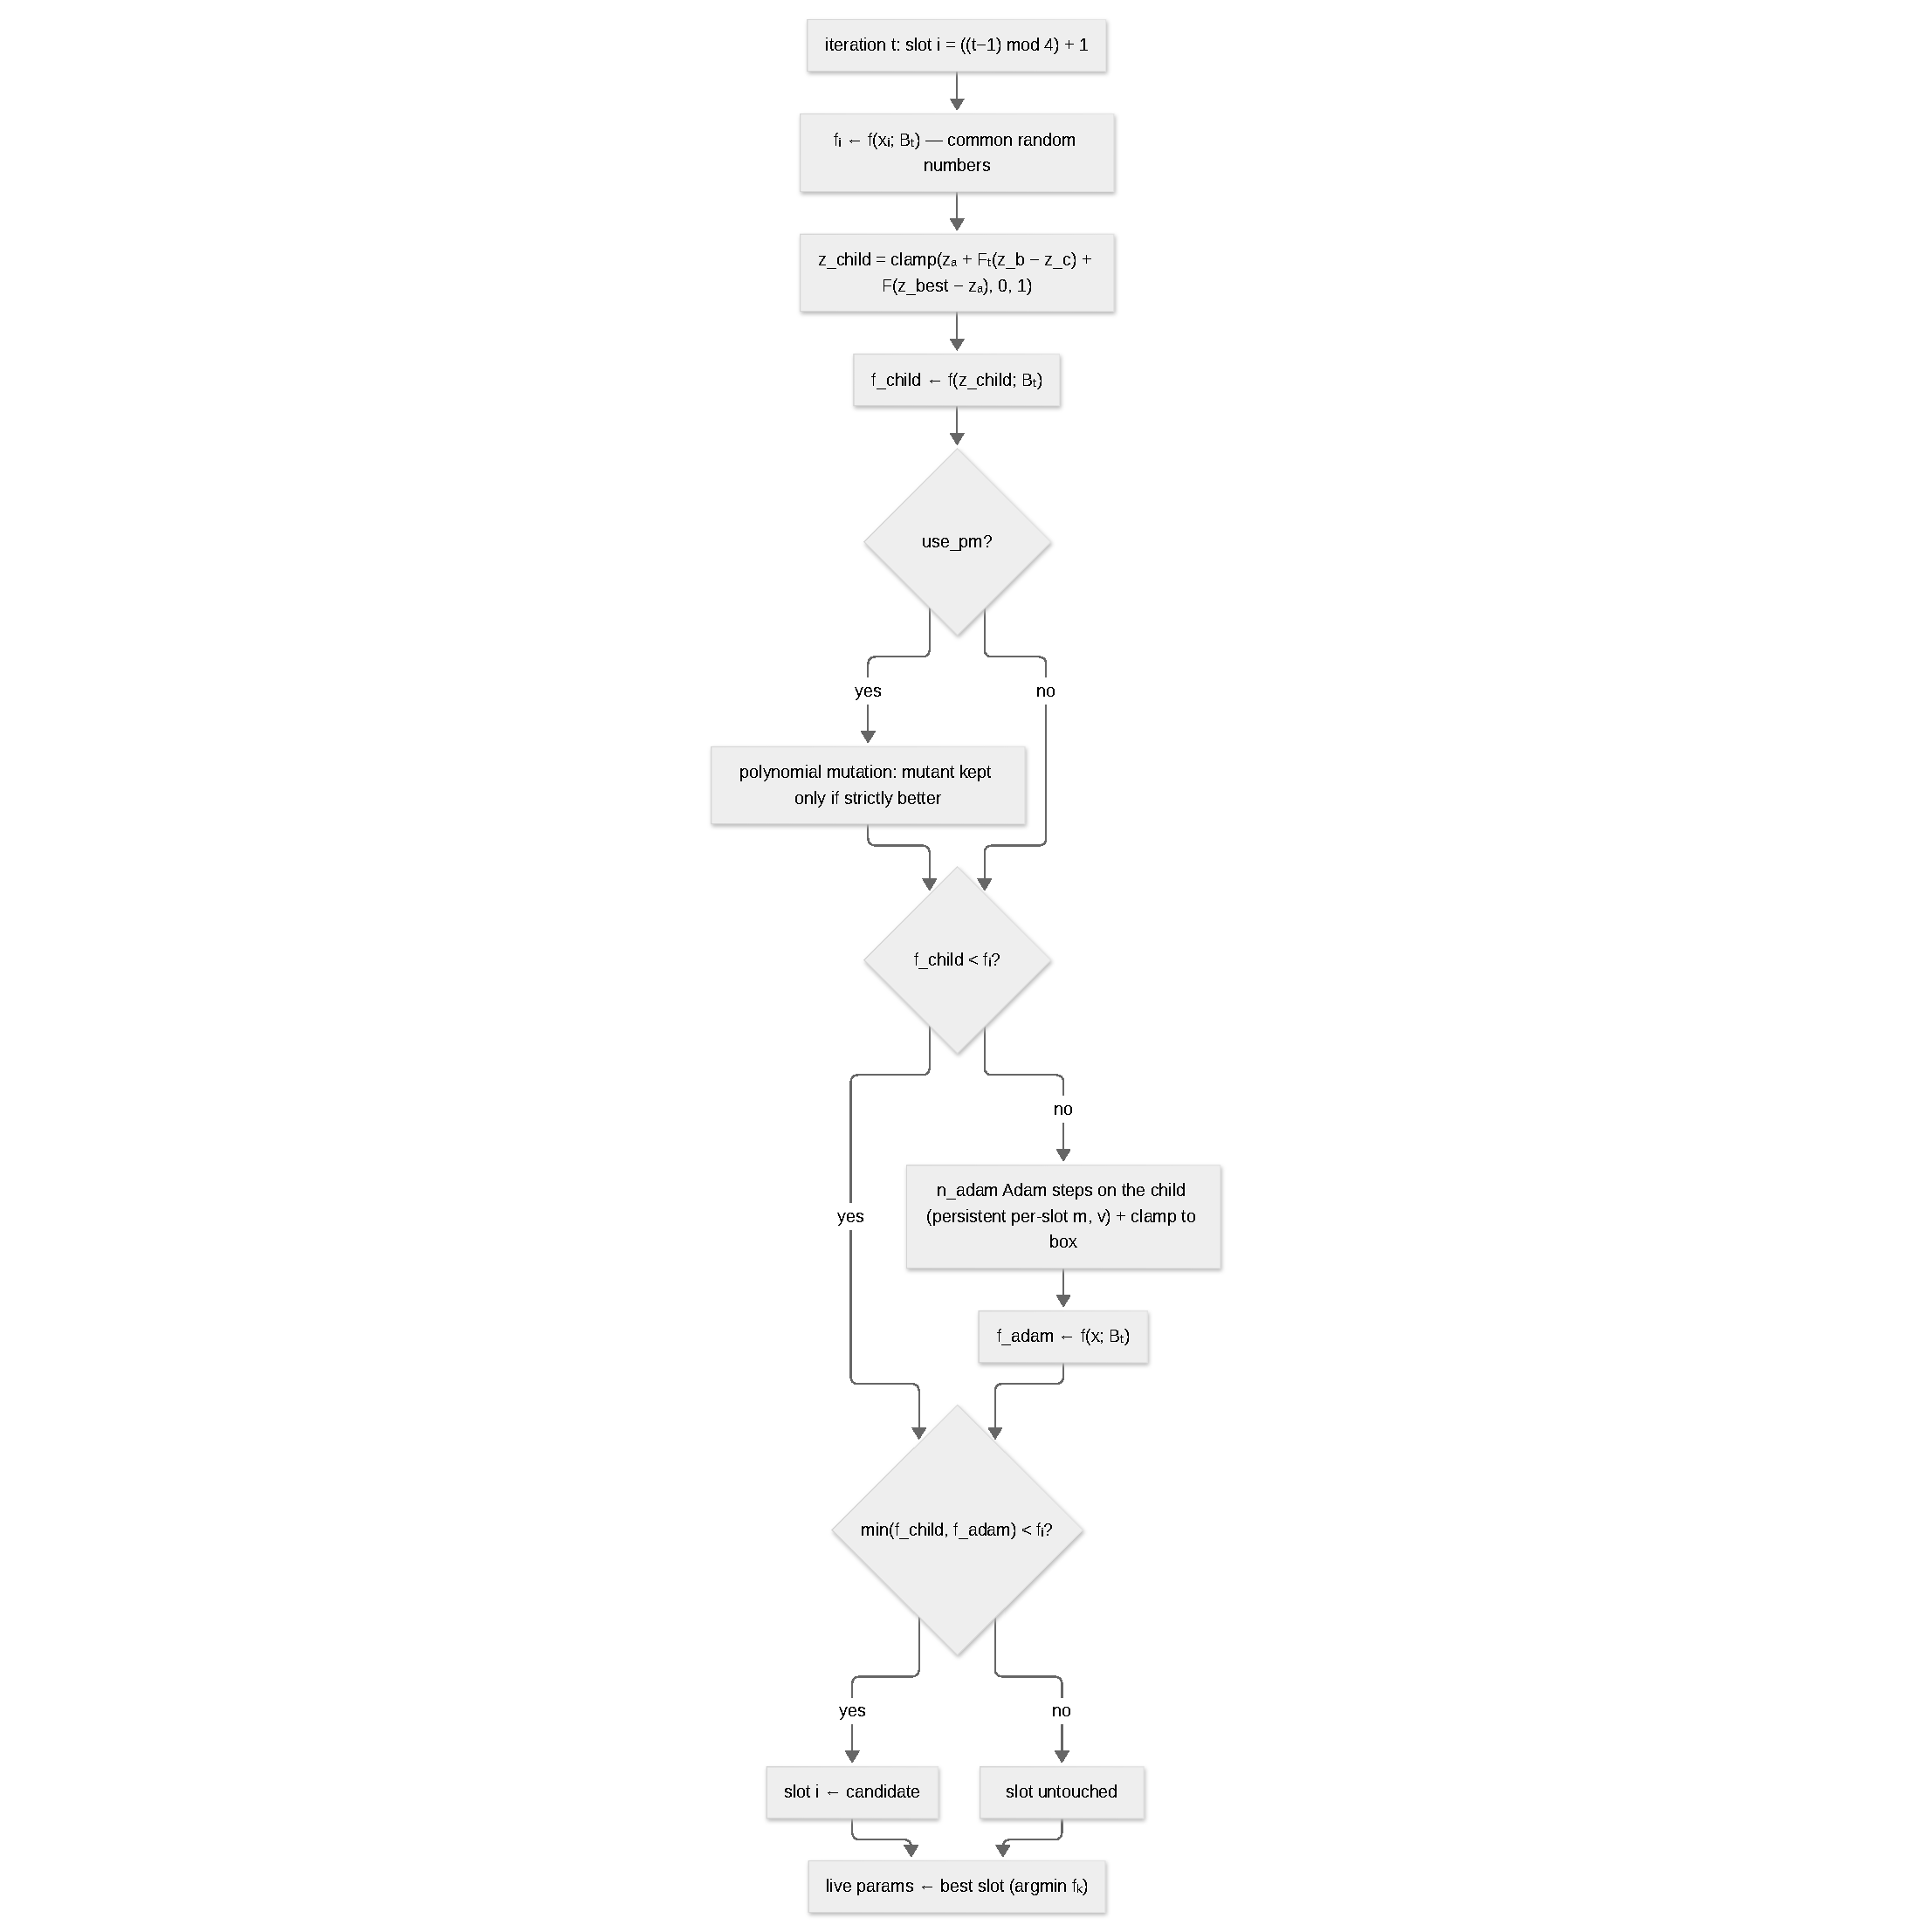
\includegraphics{../paper/figures/optimizers/eve.pdf}}
\caption{Flujo de paso de EvE: una población en régimen estable de cuatro candidatos desafía una ranura por iteración (round-robin) con un hijo de evolución diferencial; una ráfaga de Adam con estado persistente rescata al hijo solo cuando no mejora, y la selección voraz con números aleatorios comunes mantiene el mejor-observado monótono.}
\label{fig:opt-eve}
\end{figure}
EvE~\citep{raj_eve_2026} es una \textbf{alternativa poblacional a Adam} orientada al régimen con abundante búsqueda y presupuesto restringido, un nivel por encima del entrenamiento final: rankear o podar configuraciones candidatas dentro de la búsqueda de hiperparámetros y arquitecturas. En lugar de refinar un único punto, EvE mantiene una población en régimen estable de cuatro candidatos y desafía una ranura por iteración (round-robin) con un hijo de evolución diferencial \emph{rand-to-pbest/1}; solo cuando el hijo no logra mejorar al incumbente de la ranura, EvE ejecuta una ráfaga corta de Adam estándar sobre el mismo minilote, conservando el punto refinado solo si supera al hijo. La selección es voraz, de modo que el mejor-observado es monótono no creciente en objetivos deterministas, y como los gradientes se usan solo como un rescate dirigido, el costo por iteración se mantiene dentro de un factor constante de un paso de Adam sin importar la dimensión.

Toda la búsqueda interna ocurre en el cubo unitario $z \in [0,1]^n$ mediante la aplicación afín $\mathbf{x} = \mathbf{x}_l + \mathbf{z} \odot (\mathbf{x}_u - \mathbf{x}_l)$, de modo que un paso de tamaño fijo nunca sobrepasa las coordenadas de rango estrecho ni se queda corto en las de rango amplio. La población se inicializa por proximidad — un ancla con tres perturbaciones gaussianas, $\sigma = 0.1$ — anclada en los pesos iniciales del propio modelo (el precedente LoRA del artículo), con la caja de búsqueda por tensor centrada en el ancla con la semianchura Kaiming $\sqrt{6/\mathrm{fan\_in}}$. Cada iteración extrae tres donantes distintos $a, b, c \ne i$ y construye el hijo con un peso de diferencia perturbado (el jitter se aplica solo al término de diferencia; la atracción hacia pbest usa el $F$ sin perturbar):
\begin{align}
z_{\text{hijo}} &= \operatorname{clamp}\big(z_a + F_t (z_b - z_c) + F (z_{\text{pbest}} - z_a),\ 0,\ 1\big), &
F_t &= F\big(1 + \gamma (u - \tfrac{1}{2})\big), \quad u \sim U(0,1),
\end{align}
con $F = 0.5$ y $\gamma = 10^{-4}$. Una mutación polinomial opcional (PM; desactivada por defecto para el entrenamiento de redes, ya que un empujón de una sola coordenada esencialmente nunca gana su compuerta de aceptación/rechazo a escala de red) perturba exactamente un gen con tasa $p = 1/n$ e índice de distribución $\eta = 20$, con la perturbación acotada y autoescalada a la distancia a cada frontera:
\begin{align}
z_d &\leftarrow z_d + \delta_q (z_u - z_l)_d, &
\delta_q &=
\begin{cases}
\bigl[2r + (1 - 2r)(1 - \delta_1)^{\frac{1}{\eta+1}}\bigr]^{\frac{1}{\eta+1}} - 1, & r \le 0.5,\\[2pt]
1 - \bigl[2(1 - r) + 2(r - 0.5)(1 - \delta_2)^{\frac{1}{\eta+1}}\bigr]^{\frac{1}{\eta+1}}, & r > 0.5,
\end{cases}
\end{align}
con $\delta_1 = (z_d - z_l)/(z_u - z_l)$, $\delta_2 = (z_u - z_d)/(z_u - z_l)$ y $r \sim U(0,1)$. Cuando el hijo (posiblemente mutado) no supera el valor de la ranura, EvE ejecuta $n_{\text{adam}}$ pasos de Adam estándar sobre él \emph{en coordenadas reales}, con el weight decay L2 clásico plegado en el gradiente antes de la actualización de momentos (el Adam estándar de PyTorch, no la regla desacoplada de AdamW) y cada iterado reclampado a la caja:
\begin{align}
g_t &= \nabla_{\mathbf{x}} f(\mathbf{x}_{t-1}; B_t) + \lambda \mathbf{x}_{t-1}, &
m_t &= \beta_1 m_{t-1} + (1 - \beta_1) g_t, &
v_t &= \beta_2 v_{t-1} + (1 - \beta_2) g_t^2, \\
\widehat{m}_t &= \frac{m_t}{1 - \beta_1^t}, &
\widehat{v}_t &= \frac{v_t}{1 - \beta_2^t}, &
\mathbf{x}_t &= \operatorname{clamp}\Big(\mathbf{x}_{t-1} - \eta_{lr} \frac{\widehat{m}_t}{\sqrt{\widehat{v}_t} + \epsilon},\ \mathbf{x}_l,\ \mathbf{x}_u\Big),
\end{align}
con $\beta_1 = 0.9$, $\beta_2 = 0.999$, $\epsilon = 10^{-8}$. Cada ranura de la población conserva su propio estado persistente $(m, v, t)$ durante toda la ejecución, de modo que las ráfagas de respaldo forman una trayectoria de Adam continua en lugar de arranques en frío repetidos. Cada evaluación de una iteración — la actualización de la ranura, el hijo y toda la ráfaga de respaldo — se puntúa sobre un único minilote recién extraído $B_t$ (números aleatorios comunes), y un candidato reemplaza al incumbente solo si es estrictamente mejor en ese mismo lote. En esta implementación, los sufijos compartidos por grupo \texttt{lr\_*}, \texttt{wd\_*}, \texttt{betas\_*} y \texttt{eps\_*} configuran el respaldo Adam por grupo de parámetros (\texttt{wd\_*} es el término L2 $\lambda$ dentro de $g_t$), los parámetros vivos del modelo contienen siempre la mejor ranura entre pasos, y el paso se basa en closure: el trainer reevalúa el lote actual sobre cada punto candidato dentro de \texttt{optimizer.step()}, razón por la cual EvE requiere \texttt{gradient\_accumulation\_steps: 1} y no está disponible para SBERT.

\begin{algorithm}[H]
\caption{EvE (Evolutionary Explorer)}
\label{alg:eve}
\begin{algorithmic}[1]
\Require Objetivo $f$ con cotas $\mathbf{x}_l, \mathbf{x}_u$, iteraciones $T$, peso DE $F$, jitter $\gamma$, jitter de inicialización $\sigma$, índice PM $\eta$, pasos de respaldo $n_{\text{adam}}$, LR del respaldo $\eta_{lr}$, decaimiento L2 $\lambda$, semilla $s$, USE\_PM
\Ensure Mejor punto $\arg\min_k z_k$ y valor $\min_k f_k$
\State $z_1 \sim U(0,1)^n$ (ancla: los pesos iniciales); $z_k \gets \operatorname{clamp}(z_1 + \sigma\epsilon_k, 0, 1)$, $\epsilon_k \sim \mathcal{N}(0, I_n)$, $k = 2,3,4$ \Comment{Inicialización por proximidad}
\State $f_k \gets f(\mathbf{x}_l + z_k \odot (\mathbf{x}_u - \mathbf{x}_l))$ para $k = 1,\dots,4$; $\text{estado}_k \gets (\mathbf{0}, \mathbf{0}, 0)$ \Comment{Momentos de Adam persistentes}
\For{$t = 1, \ldots, T$}
    \State $i \gets ((t - 1) \bmod 4) + 1$ \Comment{Ranura objetivo round-robin}
    \State extraer minilote $B_t$; $f_i \gets f(\mathbf{x}_i; B_t)$ \Comment{Números aleatorios comunes}
    \State extraer $a, b, c$ distintos en $\{1,\dots,4\} \setminus \{i\}$; $F_t \gets F(1 + \gamma(u - 0.5))$, $u \sim U(0,1)$
    \State $z_{\text{hijo}} \gets \operatorname{clamp}(z_a + F_t(z_b - z_c) + F(z_{\text{pbest}} - z_a), 0, 1)$
    \State $f_{\text{hijo}} \gets f(z_{\text{hijo}}; B_t)$
    \If{USE\_PM} \Comment{Compuerta de aceptación/rechazo propia de PM}
        \State $z_{\text{mut}} \gets \operatorname{PM}(z_{\text{hijo}}, \eta)$; $f_{\text{mut}} \gets f(z_{\text{mut}}; B_t)$
        \If{$f_{\text{mut}} < f_{\text{hijo}}$} $z_{\text{hijo}}, f_{\text{hijo}} \gets z_{\text{mut}}, f_{\text{mut}}$ \EndIf
    \EndIf
    \If{$f_{\text{hijo}} < f_i$}
        \State $z_{\text{cand}}, f_{\text{cand}} \gets z_{\text{hijo}}, f_{\text{hijo}}$
    \Else
        \State $\mathbf{x} \gets \mathbf{x}_l + z_{\text{hijo}} \odot (\mathbf{x}_u - \mathbf{x}_l)$
        \For{$n = 1, \ldots, n_{\text{adam}}$} \Comment{Respaldo Adam dirigido}
            \State $\mathbf{x} \gets \operatorname{AdamStep}(\mathbf{x}, \nabla_{\mathbf{x}} f(\mathbf{x}; B_t), \eta_{lr}, \lambda, \text{estado}_i)$; \quad $\mathbf{x} \gets \operatorname{clamp}(\mathbf{x}, \mathbf{x}_l, \mathbf{x}_u)$
        \EndFor
        \State $z_{\text{adam}} \gets (\mathbf{x} - \mathbf{x}_l)/(\mathbf{x}_u - \mathbf{x}_l)$; \quad $f_{\text{adam}} \gets f(z_{\text{adam}}; B_t)$
        \State $(z_{\text{cand}}, f_{\text{cand}}) \gets \arg\min_{(z, f) \in \{(z_{\text{hijo}}, f_{\text{hijo}}),\, (z_{\text{adam}}, f_{\text{adam}})\}} f$
    \EndIf
    \If{$f_{\text{cand}} < f_i$} $z_i \gets z_{\text{cand}}$; \quad $f_i \gets f_{\text{cand}}$ \Comment{Selección voraz} \EndIf
\EndFor
\State \Return $\arg\min_k z_k$, $\min_k f_k$
\end{algorithmic}
\end{algorithm}

\paragraph{Contras.}
\begin{itemize}[leftmargin=*]
\item Quedan aproximadamente un punto de exactitud (MNIST) y 9--11\% de pérdida relativa (ajuste fino LoRA) por detrás de Adam a presupuesto de evaluación igualado; el artículo no reclama superioridad en la etapa final.
\item 13$\times$ el conteo de parámetros vivos en almacenamiento total (cuatro copias de población más ocho copias de momentos persistentes) frente al 4$\times$ de Adam; el multiplicador pico medido en GPU es menor (2,95$\times$) pero fijo e independiente de la dimensión.
\item Su tasa de aprendizaje no se transfiere desde la de Adam y requiere su propia búsqueda (3--100$\times$ mayor según la tarea); la población de cuatro miembros muestra la mayor varianza entre semillas de los nueve métodos comparados.
\item Paso basado en closure: el trainer reevalúa el lote dentro de \texttt{optimizer.step()}, por lo que la acumulación de gradientes no está soportada y el bucle SBERT (\texttt{fit} de sentence-transformers) no puede alojarlo; la mutación polinomial es un costo puro a escala de red y está desactivada por defecto.
\end{itemize}

\paragraph{Ventajas.}
\begin{itemize}[leftmargin=*]
\item Mejor-observado monótono por construcción en objetivos deterministas (selección voraz de aceptar solo si es estrictamente mejor), con costo por iteración dentro de un factor constante de un paso de Adam sin importar la dimensión.
\item Gana o empata con Adam en el 76\% de las 70 celdas (problema, dimensión) de los siete problemas sintéticos escalables hasta $10^6$ variables, de forma más decisiva en los multimodales.
\item Termina presupuestos de evaluación igualados 1,7--3,9$\times$ más rápido en tiempo de reloj en entrenamiento real (una MLP sobre MNIST y ajuste fino LoRA de un modelo de 1.500 millones de parámetros), intercambiando una cantidad modesta de calidad final por velocidad.
\item Dentro de successive halving, completa búsquedas de hiperparámetros y arquitecturas 3,1--3,5$\times$ más rápido mientras rankea configuraciones candidatas con una consistencia con Adam comparable a la que Adam tiene consigo mismo entre semillas ($\tau$ de Kendall de 0,66--0,69).
\end{itemize}

\paragraph{EA4LLM (Estrategias Evolutivas para Modelos de Lenguaje Grandes).}
\begin{figure}[H]
\centering
\fitfigure{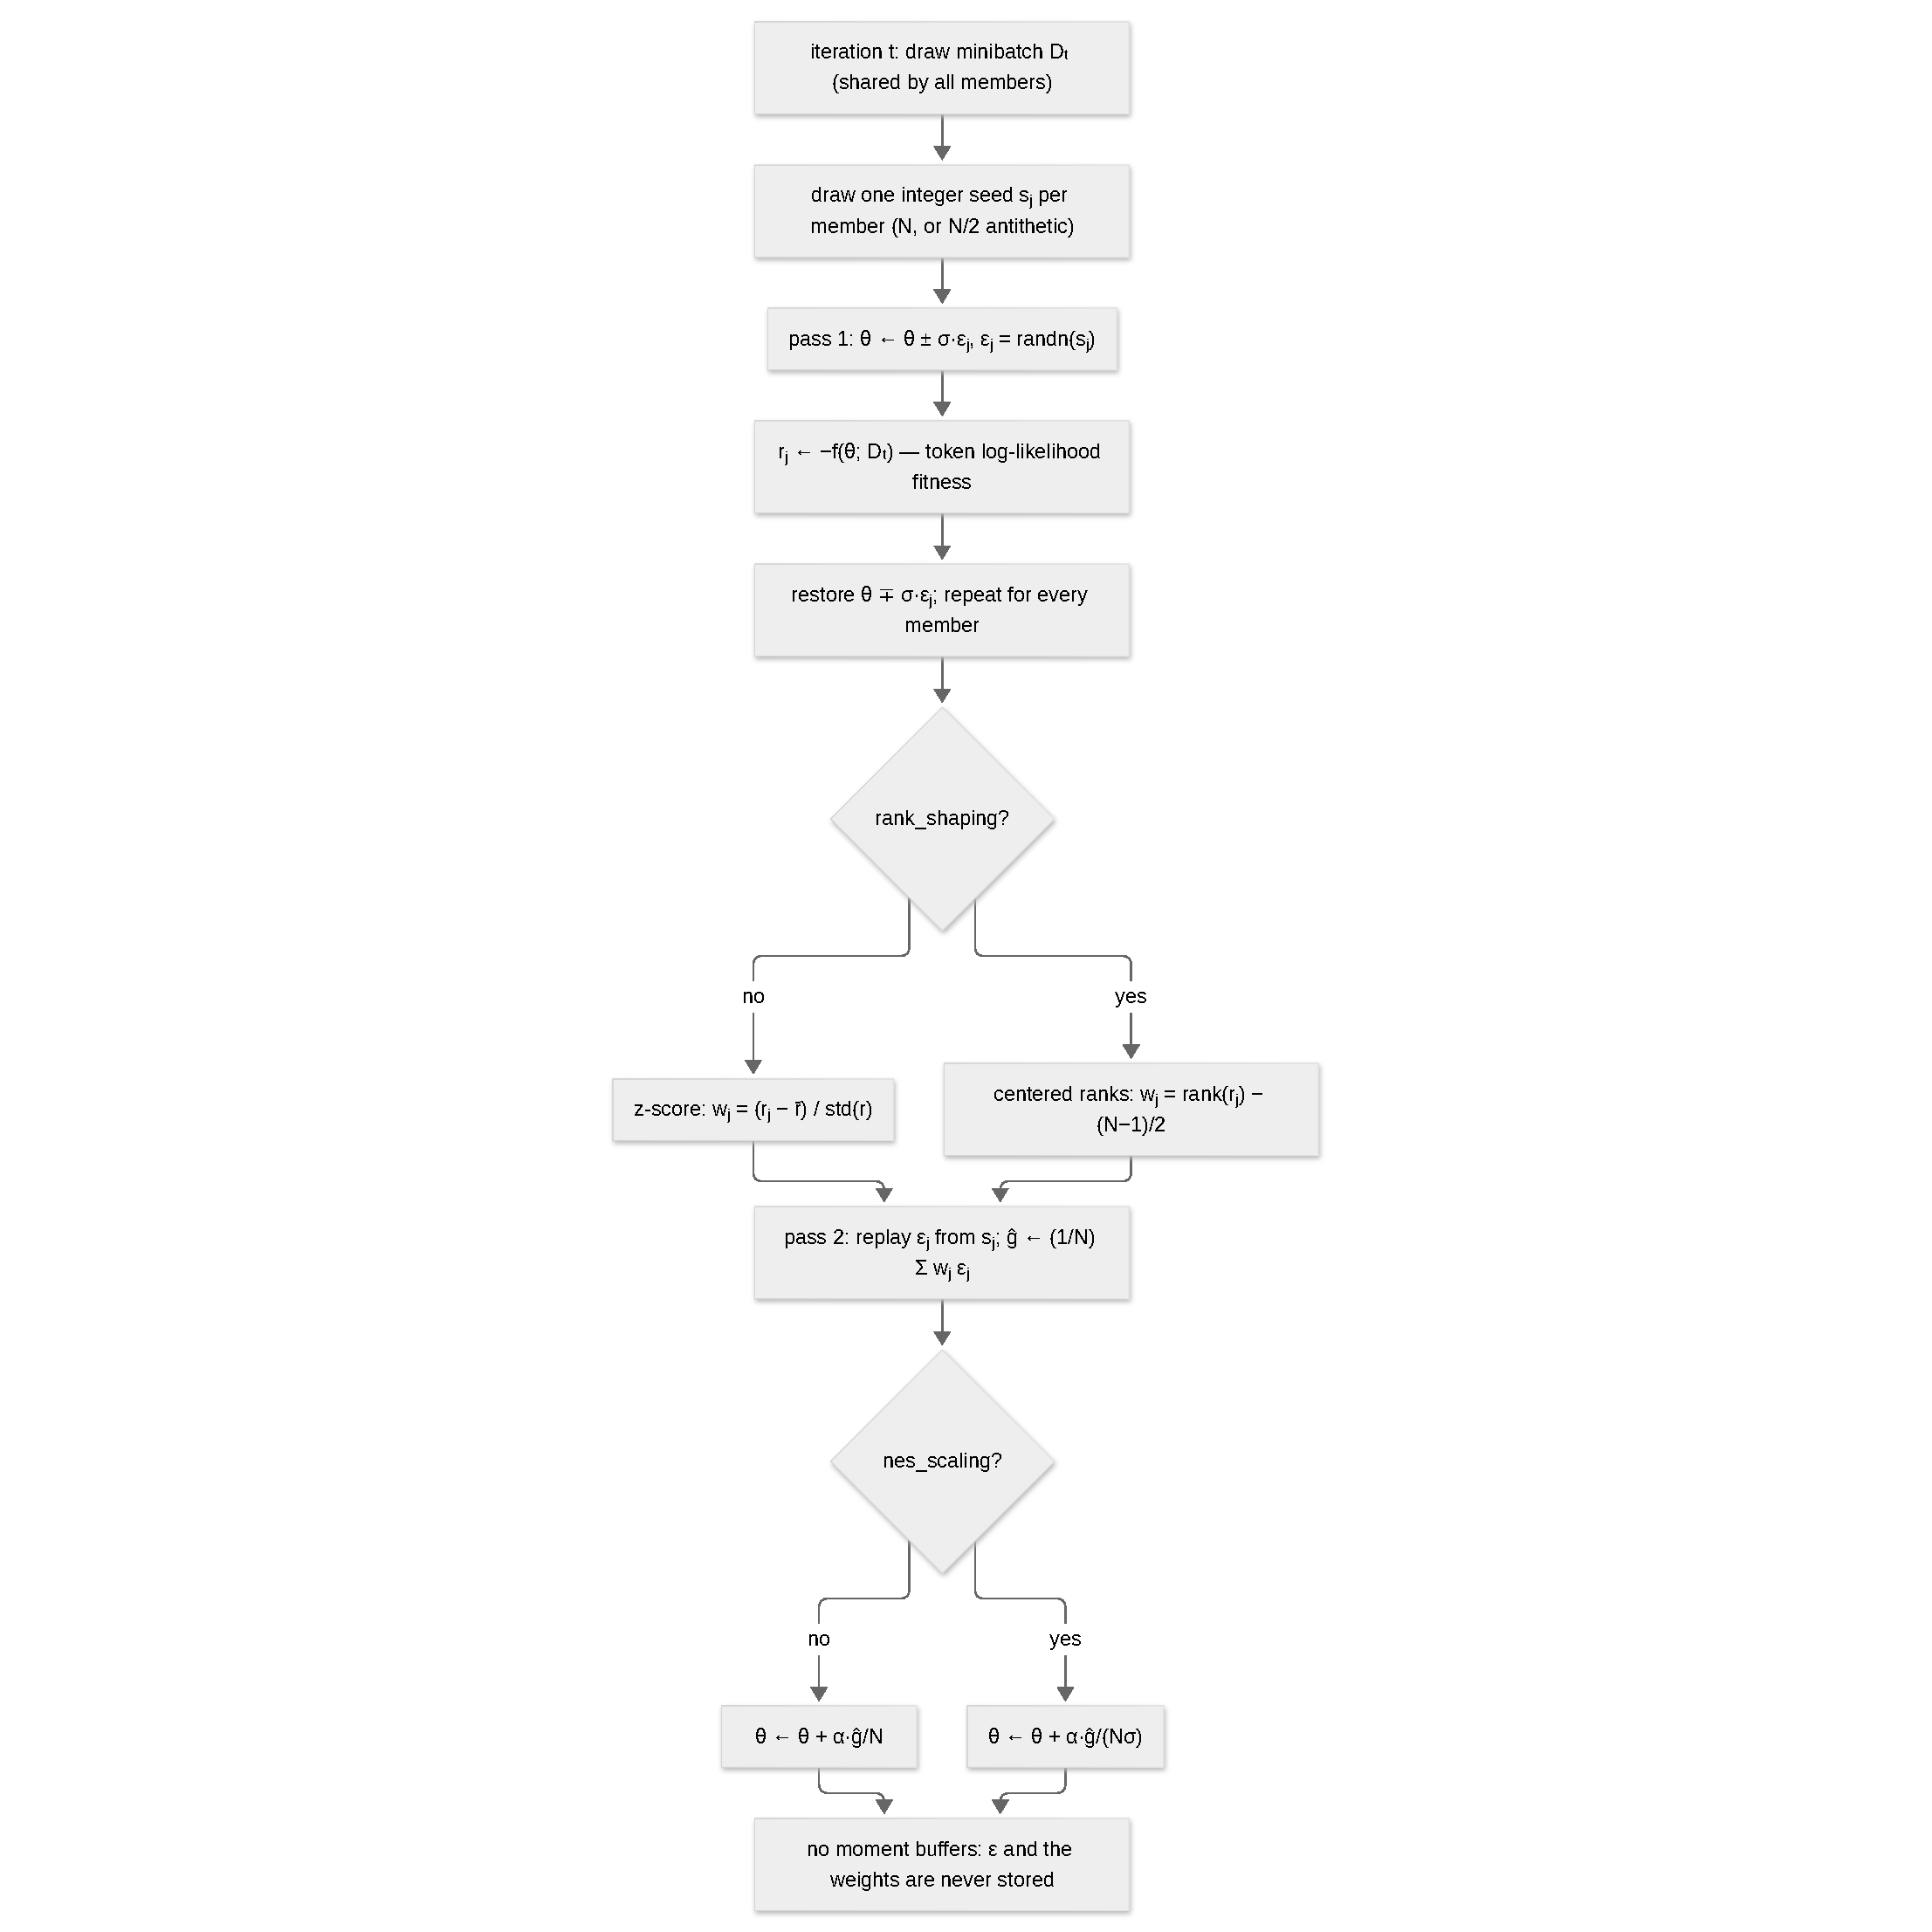
\includegraphics{../paper/figures/optimizers/ea4llm.pdf}}
\caption{Flujo de un paso de EA4LLM: cada iteración evalúa $N$ perturbaciones gaussianas de los parámetros sobre un minilote compartido por todos los miembros, las puntúa por la log-verosimilitud por token negada, convierte las recompensas en pesos z-score o de rango centrado y reproduce el mismo ruido sembrado para acumular la dirección ES --- sin gradientes ni estado del optimizador por parámetro.}
\label{fig:opt-ea4llm}
\end{figure}
EA4LLM~\citep{liu_ea4llm_2025} es una \textbf{alternativa sin gradientes a Adam} que elimina por completo la retropropagación y el estado del optimizador, y es el primer método que los autores validan para el preentrenamiento de parámetros completos de LLM desde cero, en modelos estilo Qwen3 de 0,5B a 32B parámetros. En lugar de diferenciar una pérdida, EA4LLM trata la verosimilitud del siguiente token como una aptitud de caja negra y estima una dirección de descenso a partir de una población de perturbaciones gaussianas. La aptitud es la log-probabilidad media por token del siguiente token verdadero, enmascarada para el relleno, que es exactamente el objetivo causal estándar salvo el signo:
\begin{align}
p_t &= \operatorname{softmax}(z_t), &
R(x;\theta) &= \frac{1}{\sum_t m_t}\sum_{t=1}^{T} m_t \log p_\theta\!\left(x_{t+1}\mid x_{\le t}\right), &
F(\theta) &= \frac{1}{|D|}\sum_{x\in D} R(x;\theta),
\end{align}
con logits $z_t$, máscara de relleno $m_t \in \{0,1\}$ y corpus $D$. Cada iteración muestrea $N$ ruidos independientes $\epsilon_j \sim \mathcal{N}(0, I)$, evalúa la aptitud perturbada $r_j = F(\theta + \sigma\epsilon_j)$ sobre un subconjunto $D_t \subset D$ de tamaño $M$ extraído uniformemente (el subconjunto es compartido por todos los miembros de la iteración, de modo que el estimador estocástico sigue siendo insesgado, $\mathbb{E}[F_M(\theta)] = F(\theta)$), y transforma las recompensas en pesos mediante normalización z-score o rangos centrados:
\begin{align}
w_j &= \frac{r_j - \bar r}{\operatorname{std}(r)}
&&\text{o}&
w_j &= \operatorname{rank}(r_j) - \frac{N-1}{2},
\end{align}
donde $\operatorname{rank}(\cdot)$ asigna $0,\dots,N-1$ tras ordenar. La dirección es la media ponderada por el ruido, opcionalmente escalada al estilo NES por $1/\sigma$, y la actualización asciende la aptitud:
\begin{align}
\hat g &= \frac{1}{N}\sum_{j=1}^{N} w_j \epsilon_j
&&\text{o}&
\hat g &= \frac{1}{N\sigma}\sum_{j=1}^{N} w_j \epsilon_j,
&&&
\theta \leftarrow \theta + \alpha \hat g .
\end{align}
El muestreo antitético evalúa el par $\pm\sigma\epsilon$ de $N/2$ semillas en lugar de un signo por semilla. El runner del artículo usa $N = 30$, $\sigma = 10^{-3}$, $\alpha = 5\times 10^{-4}$ y $M = 5000$ muestras de evaluación por iteración ($T = 1000$ iteraciones, micro-lote 16, longitud máxima de secuencia 256); el muestreo antitético, el shaping por rangos, el escalado NES $1/\sigma$, los multiplicadores agrupados/por capas y los programas de decaimiento del tamaño de paso están todos \emph{desactivados} en esas ejecuciones, y el Apéndice~A.1 afirma que el algoritmo desplegado elimina directamente los operadores agrupados y los multiplicadores. En esta implementación el paso se basa en closure: el minilote actual del trainer proporciona $D_t$ y la pérdida se niega para formar la aptitud, el \texttt{lr\_*} compartido por grupo es el tamaño de paso $\alpha$, y \texttt{wd\_*} aplica un decaimiento multiplicativo desacoplado antes del movimiento ES (una extensión por consistencia con el repositorio --- el artículo no define weight decay). El ruido se regenera a partir de una semilla entera por miembro en una segunda pasada, por lo que el conjunto completo de ruido nunca se almacena: el estado del optimizador es O(1) y no existen búferes de momentos. Como EvE, EA4LLM requiere \texttt{gradient\_accumulation\_steps: 1} y no está disponible para SBERT (el closure no puede coexistir con el bucle de ajuste de SBERT), y AMP no está soportado en la ruta de closure.

\begin{algorithm}[H]
\caption{EA4LLM (Estrategias Evolutivas de Orden Cero)}
\label{alg:ea4llm}
\begin{algorithmic}[1]
\Require Parámetros $\theta$, aptitud $F$ (pérdida negada), iteraciones $T$, población $N$, escala de ruido $\sigma$, tamaño de paso $\alpha$, tamaño del subconjunto $M$, normalización (z-score o rangos), semilla $s$, USE\_ANTITHETIC, USE\_RANK, USE\_NES
\Ensure Parámetros optimizados $\theta_T$
\State sembrar el generador persistente con $s$
\For{$t = 1, \ldots, T$}
    \State extraer minilote $D_t \subset D$, $|D_t| = M$ \Comment{Compartido por todos los miembros}
    \State extraer semillas $\{s_j\}_{j=1}^{N/2}$ (antitético) o $\{s_j\}_{j=1}^{N}$
    \State $\text{recompensas} \gets [\,]$ \Comment{Pasada 1: perturbar, evaluar, restaurar}
    \For{cada semilla $s_j$ y signo $\pm$ (o un único signo)}
        \State $\epsilon \gets \operatorname{randn}(s_j)$; \quad $\theta \gets \theta \pm \sigma\epsilon$; \quad $r \gets -f(\theta; D_t)$; \quad $\theta \gets \theta \mp \sigma\epsilon$
        \State añadir $r$ a recompensas
    \EndFor
    \State $w \gets$ z-score(recompensas) o rangos centrados(recompensas)
    \State $g \gets 0$ \Comment{Pasada 2: reproducir el mismo ruido}
    \For{cada semilla $s_j$ y signo $\pm$ (o un único signo)}
        \State $\epsilon \gets \operatorname{randn}(s_j)$; \quad $g \gets g + w_j (\pm\epsilon)$
    \EndFor
    \State $\theta \gets \theta + \alpha g / (N\sigma)$ si USE\_NES, si no $\theta \gets \theta + \alpha g / N$
\EndFor
\State \Return $\theta_T$
\end{algorithmic}
\end{algorithm}

\paragraph{Contras.}
\begin{itemize}[leftmargin=*]
\item Requiere $N$ evaluaciones forward por paso (30 en el artículo), por lo que la eficiencia de muestreo queda por detrás de los métodos de primer orden y la varianza del estimador es mayor; el artículo reporta sensibilidad a $N$, $\sigma$, $\alpha$ y a la elección de normalización.
\item No hay gradiente disponible, de modo que las rutas de recorte de gradiente y AMP no aplican: el arnés de closure del trainer rechaza \texttt{use\_amp}, exige \texttt{gradient\_accumulation\_steps: 1} y el bucle SBERT no puede alojarlo. Cada evaluación además paga una pasada backward a través del closure compartido aunque ES la descarte.
\item A presupuestos de evaluación igualados el artículo no reclama calidad final superior a Adam; su argumento es la memoria (>4$\times$ de reducción con $\ge$4B parámetros) y la viabilidad sin gradientes, con el muestreo antitético, el shaping por rangos y el escalado NES desactivados en sus propias ejecuciones a gran escala.
\item Como el z-score hace que la magnitud de la actualización sea independiente de $\sigma$ y de la escala del gradiente, $\alpha$ debe ajustarse por tarea en lugar de transferirse desde Adam.
\end{itemize}

\paragraph{Ventajas.}
\begin{itemize}[leftmargin=*]
\item Estado del optimizador nulo: sin momentos y sin copias de población, por lo que el artículo mide 60,01 frente a 137,61~GB en 8B y 137,61 frente a 431,76~GB en 32B contra Adam.
\item Proporciona el primer preentrenamiento ES estable de parámetros completos desde cero en 0,5B--32B, con curvas de pérdida que descienden de forma sostenida (Figura~1) y sin cálculo de gradientes.
\item Agnóstico a la arquitectura: la aptitud solo necesita una pasada forward y una probabilidad, por lo que los operadores no diferenciables se vuelven entrenables.
\item La aptitud submuestreada es un estimador insesgado de la aptitud sobre el corpus completo, y la reproducción sembrada en dos pasadas hace el ruido reproducible manteniendo el estado del optimizador en O(1).
\end{itemize}

